\documentclass[11pt]{amsart}


\usepackage{geometry}                % See geometry.pdf to learn the layout options. There are lots.
\geometry{a4paper}                   % ... or a4paper or a5paper or ...
%\geometry{landscape}                % Activate for for rotated page geometry
\usepackage[parfill]{parskip}    % Activate to begin paragraphs with an empty line rather than an indent
\usepackage{enumitem}
\usepackage{graphicx}
\usepackage{amssymb}
\usepackage{amsmath}
\usepackage{cancel}
\usepackage{tikz}
\usepackage{epstopdf}
\DeclareGraphicsRule{.tif}{png}{.png}{`convert #1 `dirname #1`/`basename #1 .tif`.png}
\usepackage{breqn}

\usetikzlibrary{calc,intersections,through,backgrounds,arrows,decorations.markings}

\tikzset{
  coordsys/.pic={
    \draw[->] (0,0) -- ++(6mm,0pt);
    \draw[->] (0,0) -- ++(0pt,6mm);
  },
  myarr/.style={decoration={
      markings,
      mark=between positions 0 and 1 step 2mm with {\arrow{stealth}},
    },
    postaction=decorate
  },
}

\title{Econ 210C Problem Set \# 2}
\author{Nathaniel Bechhofer}
%\date{}                                           % Activate to display a given date or no date

\begin{document}




\maketitle

\section{Investment and the Housing Market}

\subsection*{(a)}
\begin{enumerate}
	\item $I = \psi (P)$: Gross investment in housing is an increasing function of the price of houses. This specification implies that housing investment can be interpreted as the supply of new housing. 
	\item $r + \delta = (R + \dot{P})/P$: This implies that the costs of investing into a house, namely forgone investment income and depreciation are equal to the benefits, namely rental payments and capital gains. 
	\item $R = R(H)$: Rental cost is a decreasing function of the size of the housing stock. 
	\item $\dot{H} = I - \delta H$: The housing stock can change in two ways, housing investment and depreciation.
\end{enumerate}

\subsection*{(b)}

We merely substitute to obtain

\begin{align*}
\dot{H} &= \psi(P) - \delta H \\
r + \delta &= (R(H) + \dot{P}) / P
\end{align*}




\begin{figure}[htbp]
\begin{center}
\begin{tikzpicture}[x=3cm,y=3cm]
\draw [name path=A--B]
(0.2,0.5) -- 
(1.8,1.5) node[right] {$\dot{H} = 0$};
\draw[name path=C--D]
(0.2,1.5) to[bend right] 
(1.8,0.5) node[right] {$\dot{P} = 0$};
\path [name intersections={of=A--B and C--D,by=E}];
\node [fill=red,inner sep=1pt] at (E) {};
\draw[->]
  (-0.1,0) -- (2,0) node[right] {$H$};
\draw[->]
  (0,-0.1) -- (0,2) node[above] {$P$};
\draw[myarr]
  (0.2,1) -- 
  (E);
\draw[myarr]
  (1.6,0.8) -- 
  (E);
\path
  pic[yscale=-1] at (0.3,1) {coordsys}
  pic[xscale=-1] at (1.7,1) {coordsys}
  pic at (0.8,1.7) {coordsys}
  pic[rotate=180] at (1.5,0.3) {coordsys};
\end{tikzpicture}
\caption{Phase diagram for 1c}
\label{1c}
\end{center}
\end{figure}

\subsection*{(d)}

Rewriting the equation for $\dot{P}$ gives 
\[
\dot{P} + R(H) = P (r + \delta)
\]
implying an increase in $r$ must increase $R(H)$ correspondingly given $\dot{P} = 0$. 
Since $R$ is a decreasing function of $H$, we have that $H$ decreases and the $\dot{P} = 0$ locus shifts to the left.

\subsection*{(e)}

If we go from $r$ to $r^{*}$, where $r < r^{*}$, then $P$ immediately drops to the level $\frac{R(H)}{r^{*} + \delta}$, as the higher opportunity cost of investing in housing reduces the quantity of housing investment.
As housing investment decreases, the quantity of housing stock decreases gradually until $R(H)$ goes up to the $\dot{P}=0$ point. 
So we have that $H$ moves gradually down to the new steady state, $P$ drops immediately then rises to its new but lower level, $I$ drops immediately then rises to its new lower level, and $R$ rises gradually to its new steady state level.

\begin{figure}[htbp]
\begin{center}
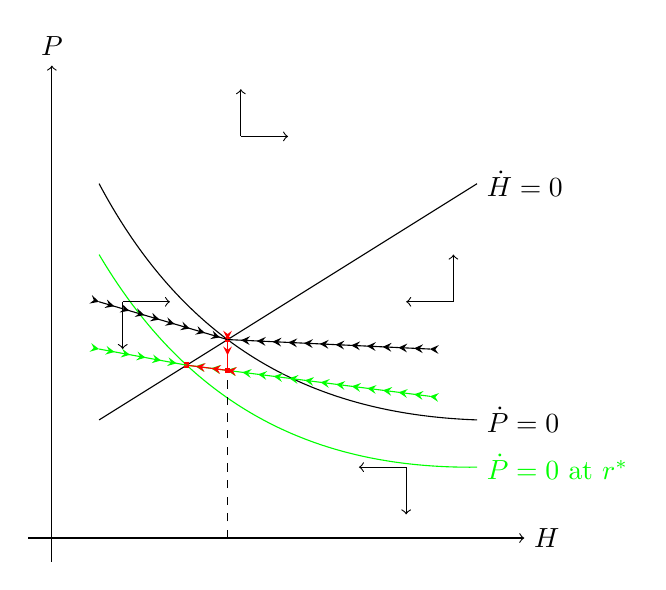
\begin{tikzpicture}[x=3cm,y=3cm]
\draw [name path=A--B]
(0.2,0.5) -- 
(1.8,1.5) node[right] {$\dot{H} = 0$};
\draw[name path=C--D]
(0.2,1.5) to[bend right] 
(1.8,0.5) node[right] {$\dot{P} = 0$};
\path [name intersections={of=A--B and C--D,by=E}];
\draw[name path=F--G, color=green]
(0.2,1.2) to[bend right] 
(1.8,0.3) node[right] {$\dot{P} = 0$ at $r^{*}$};
\path [name intersections={of=A--B and F--G,by=H}];
\node [fill=red,inner sep=1pt] at (E) {};
\draw[->]
  (-0.1,0) -- (2,0) node[right] {$H$};
\draw[->]
  (0,-0.1) -- (0,2) node[above] {$P$};
\draw [dashed, name path=Hdash] 
  ($(-0.1,0)!(E)!(2,0)$) -- (E);
\node [fill=red,inner sep=1pt] at (H) {};
\draw[myarr]
  (0.2,1) -- 
  (E);
\draw[myarr]
  (1.6,0.8) -- 
  (E);
\draw[myarr, color=green]
  (0.2,0.8) -- 
  (H);
\draw[myarr, color=green, name path=J--K]
  (1.6,0.6) -- 
  (H);
\path [name intersections={of=Hdash and J--K,by=J}];
\node [fill=red,inner sep=1pt] at (J) {};
\draw[myarr, color=red]
  (E) -- 
  (J);
\draw[myarr, color=red]
  (J) -- 
  (H);
\path
  pic[yscale=-1] at (0.3,1) {coordsys}
  pic[xscale=-1] at (1.7,1) {coordsys}
  pic at (0.8,1.7) {coordsys}
  pic[rotate=180] at (1.5,0.3) {coordsys};
\end{tikzpicture}
\caption{Change in the real interest rate}
\label{1e}
\end{center}
\end{figure}

\subsection*{(f)}

$P$ will still drop immediately, but to a level higher than $\frac{R(H)}{r^{*} + \delta}$, because we still have that the higher opportunity cost of investing in housing reduces the quantity of housing investment.
As housing investment decreases, the quantity of housing stock decreases at first, leveling off during the period increased interest rates, after which it rises again forever back up to the original $\dot{P}=0$ point. 
So we have that $H$ moves gradually down until it starts rising again (before the increase is over) to the same steady state, $P$ drops immediately then rises back to its original level (with a discrete jump when the increase is over), $I$ drops immediately then rises back to its original level (with a discrete jump when the increase is over), and $R$ rises gradually until it levels off at the same point $H$ does, after which it gradually falls to the same steady state level.

\subsection*{(g)}

$P$ will still drop immediately, and then gradually declines further until it hits $\frac{R(H)}{r^{*} + \delta}$ (with a discrete drop when the increase hits).

$H$ declines gradually starting immediately toward the new lower steady state value. 

$I$ drops immediately, then rises to its new lower level.

$R$ increases gradually starting immediately toward the new higher steady state value.


\subsection*{(h)}

In this case, we merely have
\[
r + \delta = R(H) / P
\]
so an increase in $r$ implies an immediate fall in $P$

$P$ will drop immediately, and then rises slowly to its new steady state value. 

$H$ declines gradually; $(H,P)$ moves along the $\dot{P} = 0$ locus.

$I$ drops immediately, then rises to its new lower level.

$R$ increases gradually starting immediately toward the new higher steady state value.

\subsection*{(i)}

If people have static expectations and there is an interest rate shock, then the model matches everything in the housing crisis; prices and construction dropped rapidly, while there was little effect on rental costs.

\section{Discount Factor Shocks}

The only equation affected is the Euler equation, so we have our model:
\begin{align*}
\lambda_t &= \frac{1}{C_t} \\
\frac{C_{t+1}}{C_t} &=  E[\beta_{t+1} (1+ R_{t+1})]\\
W_t &= (1-\alpha) Z_t \left( \frac{K_{t-1}}{L_t} \right)^\alpha \\
R_t + \delta & = \alpha Z_t \left( \frac{K_{t-1}}{L_t} \right)^{\alpha-1} \\
L_t^{\frac{1}{\eta}} C_t &= W_t \\
C_t + I_t + G_t &= Z_t L_t \left(\frac{K_{t-1}}{L_t} \right)^\alpha \\
K_t &= (1-\delta) K_{t-1} + I_t
\end{align*}

We have the endogenous variables ($\lambda_t, K_t, W_t, C_t, L_t, R_t, I_t$ ) and exogenous variables ($\beta_t, Z_t, G_t)$, and so we can follow the derivation from class, only replacing the Euler equation to get the $\check{\beta_t}$ term.
\begin{align*}
\Delta \check{K_t} &= \frac{\bar{Y}}{\bar{K}} \left( 1 + \frac{1-\alpha}{\alpha + 1/\eta} \right) \check{Z_t} + \left( \frac{\alpha (1-\alpha )}{\alpha + 1/\eta}  \frac{\bar{Y_t}}{\bar{K_t}}  + \alpha \frac{\bar{Y}}{\bar{K}} - \delta  \right) \check{K_{t-1}}  \\
&+ \left( \frac{\bar{C}}{\bar{K}} + \frac{\bar{Y}}{\bar{K}} \frac{(1-\alpha)}{\alpha + 1/\eta}\right) \check{\lambda_t} - \frac{\bar{G}}{\bar{K}}\check{G_t} \\
\Delta \check{\lambda_{t+1}}  &=  - \check{\beta_{t+1}} - \frac{\alpha \frac{\bar{Y}}{\bar{K}}}{\alpha \frac{\bar{Y}}{\bar{K}} + 1 - \delta} \left[   \left( 1 + \frac{1-\alpha}{\alpha + 1/\eta} \right) \check{Z_{t+1}} + (1-\alpha) \left( \frac{\alpha}{1/\eta + \alpha} -1 \right) \check{K_t} + \frac{1-\alpha}{1/\eta + \alpha} \check{\lambda_{t+1}}  \right]
\end{align*}

By setting $\Delta \lambda_t = 0$, we have the locus of points where the marginal utility of consumption is constant.
\paragraph{\bf Locus $\Delta \lambda_t = 0$} 
\begin{equation*}
\check{\lambda_{t+1}} = -  \frac{1/\eta + \alpha}{1-\alpha} \left[  \left( \frac{\alpha \frac{\bar{Y}}{\bar{K}}}{\alpha \frac{\bar{Y}}{\bar{K}} + 1 - \delta} \right)^{-1} \check{\beta_{t+1}} +  \left( 1 + \frac{1-\alpha}{\alpha + 1/\eta} \right) \check{Z_{t+1}} + (1-\alpha) \left( \frac{\alpha}{1/\eta + \alpha} -1 \right) \check{K_t} \right] 
\end{equation*}

The phase diagram for this economy is identical to the phase diagram in the notes. 

\begin{figure}[htbp]
\begin{center}
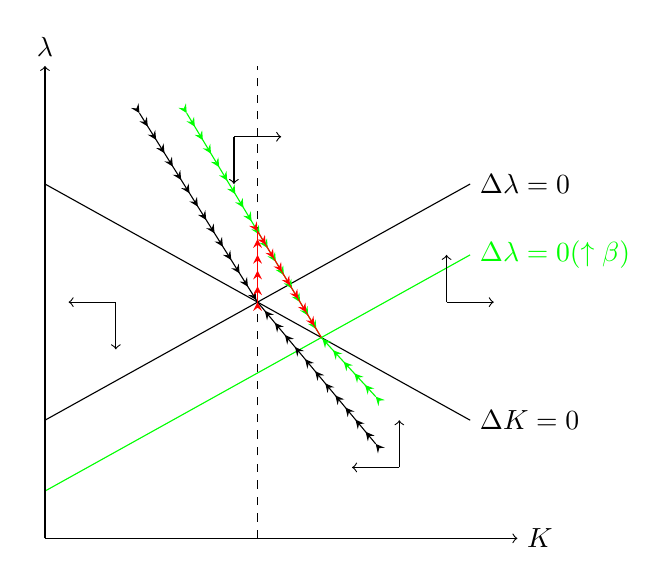
\begin{tikzpicture}[x=3cm,y=3cm]
\draw [name path=A--B]
(0,0.5) -- 
(1.8,1.5) node[right] {$\Delta \lambda = 0$};
\draw[name path=C--D]
(0,1.5) --
(1.8,0.5) node[right] {$\Delta K = 0$};
\draw[name path=F--G, color=green]
(0,0.2) --
(1.8,1.2) node[right] {$\Delta \lambda = 0 (\uparrow \beta)$};
\path [name intersections={of=A--B and C--D,by=E}];
\path [name intersections={of=C--D and F--G,by=H}];
%\node [fill=red,inner sep=1pt] at (E) {};
\draw[->]
  (0,0) -- (2,0) node[right] {$K$};
\draw[->]
  (0,-0) -- (0,2) node[above] {$\lambda$};
\draw [dashed, name path=Hdash] 
  ($(0,0)!(E)!(2,0)$) -- (E);
\draw [dashed, name path=Hdashprime] 
  (E) -- ($(0,2)!(E)!(2,2)$);
%\node [fill=red,inner sep=1pt] at (H) {};
\draw[myarr]
  (0.4, 1.8) -- 
  (E);
\draw[myarr]
  (1.4, 0.4) -- 
  (E);
\draw[myarr, color=green, name path=J--K]
  (0.6,1.8) -- 
  (H);
\draw[myarr, color=green]
  (1.4,0.6) -- 
  (H);
\path [name intersections={of=Hdashprime and J--K,by=J}];
%\node [fill=red,inner sep=1pt] at (J) {};
\draw[myarr, color=red]
  (E) -- 
  (J);
\draw[myarr, color=red]
  (J) -- 
  (H);
\path
  pic[rotate=180] at (0.3,1) {coordsys}
  pic at (1.7,1) {coordsys}
  pic[yscale=-1] at (0.8,1.7) {coordsys}
  pic[xscale=-1] at (1.5,0.3) {coordsys};
\end{tikzpicture}
\caption{Change in $\beta$}
\label{fig2}
\end{center}
\end{figure}

\begin{figure}[htbp]
\begin{center}
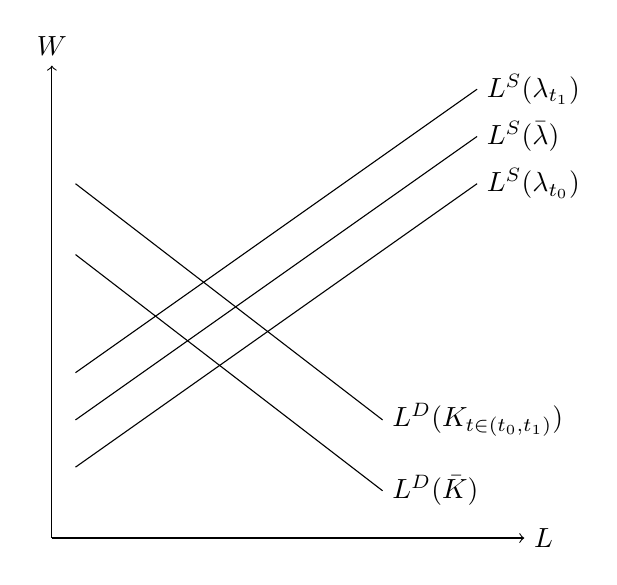
\begin{tikzpicture}[x=3cm,y=3cm]
\draw [name path=LSbar]
(0.1,0.3) -- 
(1.8,1.5) node[right] {$L^S(\lambda_{t_0})$};
\draw [name path=LS0]
(0.1,0.5) -- 
(1.8,1.7) node[right] {$L^S(\bar{\lambda})$};
\draw [name path=LStrans]
(0.1,0.7) -- 
(1.8,1.9) node[right] {$L^S(\lambda_{t_1})$};
\draw [name path=LD0]
(0.1,1.2) -- 
(1.4,0.2) node[right] {$L^D(\bar{K})$};
\draw [name path=LDtrans]
(0.1,1.5) -- 
(1.4,0.5) node[right] {$L^D(K_{t \in (t_0,t_1)})$};
\draw[->]
  (0,0) -- (2,0) node[right] {$L$};
\draw[->]
  (0,-0) -- (0,2) node[above] {$W$};

\end{tikzpicture}
\caption{Discount factor shock (temporay) labor diagram}
\label{DiscountFactorLaborDiagram}
\end{center}
\end{figure}

\begin{table}[htp]
\caption{Response to permanent $\beta$ shock}
\begin{center}
\begin{tabular}{c|c|c|c|}
& Impact & Transition & Steady State \\ \hline
$C$ & $\downarrow$ & $\uparrow$ & $\uparrow$ \\
$Y$ & $\uparrow$ & ? & $\uparrow$ \\
$I$ & $\uparrow$ & $\downarrow$ & $\uparrow$ \\
$L$ & $\uparrow$ & ? & ? \\
$W$ & $\downarrow$ & $\uparrow$ & $\uparrow$ \\
$R$ & $\uparrow$ & $\downarrow$ & $\downarrow$ \\
\end{tabular}
\end{center}
\label{default}
\end{table}

\begin{table}[htp]
\caption{Response to temporary $\beta$ shock}
\begin{center}
\begin{tabular}{c|c|c|c|c|c}
			& Impact  & Transition I          & Inflection & Transition II & Steady State  \\
		& $t=t_0$ & $t \in (t_0, t_1)$ & $t = t_1$ & $t \in (t_1, \infty)$ & $t = \infty$ \\
		\hline 
		$C$          & $\downarrow$ &   $\uparrow$      &   0      & $\downarrow$ &    0\\
		$Y$          &    $\uparrow$   &    ?    &    0    &  $\downarrow$  &      0\\
		$I$           &   $\uparrow$    &  $\downarrow$  & 0 & $\downarrow$  &    0\\
		$L$          &   $\uparrow$    &   ?      & 0     &  ? &      0\\
		$W$         & $\downarrow$ &    $\uparrow$     &    0     & $\downarrow$ &  0   \\
		$R$          &  $\uparrow$    &     $\downarrow$     &    0     & $\uparrow$  &  0 \\
		\hline
\end{tabular}
\end{center}
\label{default}
\end{table}

With more patient agents, consumption drops immediately.
Marginal utility jumps up to the new stable arm, so we know that we will have higher labor supply and investment.
Investments decreases and consumption increases as the economy approaches to the new steady state.
In the steady state, the capital stock and consumption are both higher. 
The increased labor demand from the capital stock implies higher emplyment output. 
Wages are higher and the interest rate is lower. 


For a transitory discount factor shock, marginal utility jumps up and moves so it is back on the initial stable arm when the shock ends. 
Labor supply jumps up and consumption jumps down immediately. 
The reduced consumption also means a jump in output and investment. 
Capital increases gradually. 
Increased labor supply implies lower wages; the interest rate increases.
Consumption increases as labor supply decreases during the period of the shock. 
Increased labor demand means that the effect on employment and output is ambiguous.
When the shock ends, the economy moves along the initial stable arm to the initial steady state. 


\section{News Shocks}

\begin{figure}[htbp]
\begin{center}
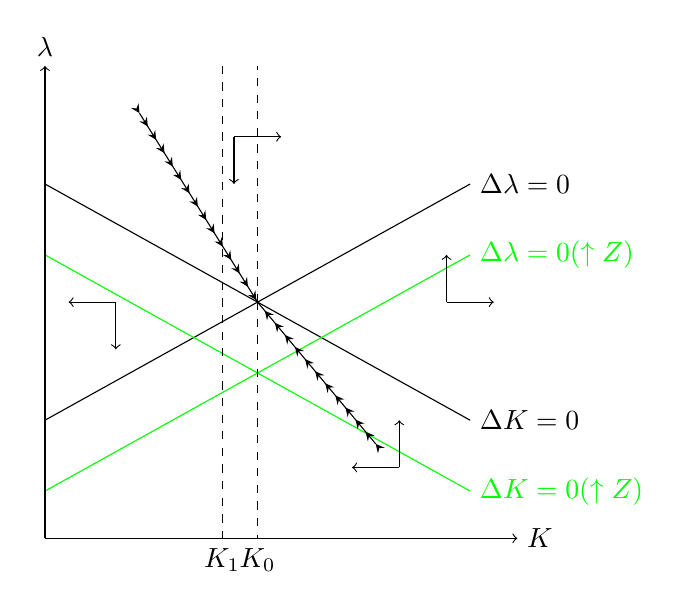
\begin{tikzpicture}[x=3cm,y=3cm]
\draw [name path=A--B]
(0,0.5) -- 
(1.8,1.5) node[right] {$\Delta \lambda = 0$};
\draw[name path=C--D]
(0,1.5) --
(1.8,0.5) node[right] {$\Delta K = 0$};
\draw[name path=F--G, color=green]
(0,0.2) --
(1.8,1.2) node[right] {$\Delta \lambda = 0 (\uparrow Z)$};
\draw[name path=J--K, color = green]
(0,1.2) --
(1.8,0.2) node[right] {$\Delta K = 0 (\uparrow Z)$};
\path [name intersections={of=A--B and C--D,by=E}];
%\node [fill=red,inner sep=1pt] at (E) {};
\draw[->]
  (0,0) -- (2,0) node[right] {$K$};
\draw[->]
  (0,-0) -- (0,2) node[above] {$\lambda$};
\draw [dashed, name path=Edash] 
  (E) -- ($(0,0)!(E)!(2,0)$)  node[below] {$K_0$};
\draw [dashed, name path=Edashprime] 
  (E) -- ($(0,2)!(E)!(2,2)$);
\draw [dashed, name path=newK] 
  (0.75,2) -- (0.75,0) node[below] {$K_1$};
%\node [fill=red,inner sep=1pt] at (H) {};
\draw[myarr]
  (0.4, 1.8) -- 
  (E);
\draw[myarr]
  (1.4, 0.4) -- 
  (E);
\path
  pic[rotate=180] at (0.3,1) {coordsys}
  pic at (1.7,1) {coordsys}
  pic[yscale=-1] at (0.8,1.7) {coordsys}
  pic[xscale=-1] at (1.5,0.3) {coordsys};
\end{tikzpicture}
\caption{News shock phase diagram}
\label{NewsShocksPhaseDiagram}
\end{center}
\end{figure}

\begin{figure}[htbp]
\begin{center}
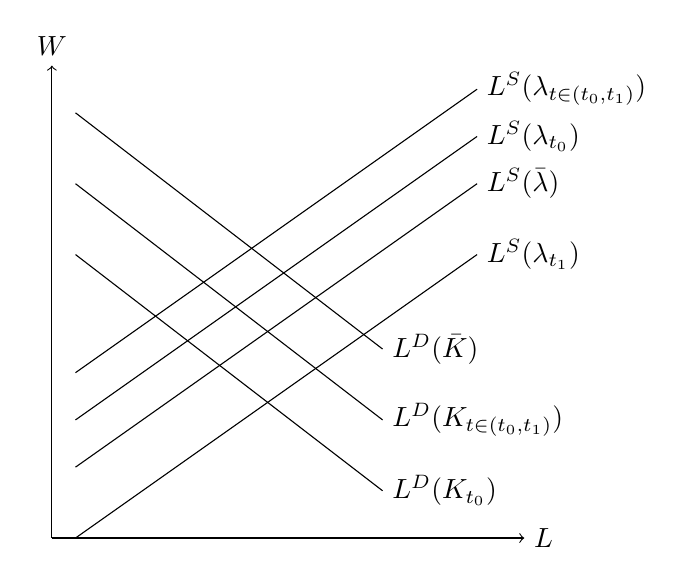
\begin{tikzpicture}[x=3cm,y=3cm]
\draw [name path=LSbar]
(0.1,0.3) -- 
(1.8,1.5) node[right] {$L^S(\bar{\lambda})$};
\draw [name path=LS0]
(0.1,0.5) -- 
(1.8,1.7) node[right] {$L^S(\lambda_{t_0})$};
\draw [name path=LStrans]
(0.1,0.7) -- 
(1.8,1.9) node[right] {$L^S(\lambda_{t \in (t_0,t_1)})$};
\draw [name path=LS1]
(0.1,0) -- 
(1.8,1.2) node[right] {$L^S(\lambda_{t_1})$};
\draw [name path=LD0]
(0.1,1.2) -- 
(1.4,0.2) node[right] {$L^D(K_{t_0})$};
\draw [name path=LDtrans]
(0.1,1.5) -- 
(1.4,0.5) node[right] {$L^D(K_{t \in (t_0,t_1)})$};
\draw [name path=LDbar]
(0.1,1.8) -- 
(1.4,0.8) node[right] {$L^D(\bar{K})$};
\draw[->]
  (0,0) -- (2,0) node[right] {$L$};
\draw[->]
  (0,-0) -- (0,2) node[above] {$W$};

\end{tikzpicture}
\caption{News shock labor diagram}
\label{NewsShocksLaborDiagram}
\end{center}
\end{figure}

Marginal utility drops to get to a path on the new stable arm when the shock comes. 
Households increase consumption in anticipation of higher output.
When the shock does not come, households decrease consumption immediately. 
The economy now moves back to the initial stable arm.
When the shock is anticipated, labor supply goes down, implying higher wages and lower employment. 
Labor demand drops due to reduced investment, as does output. 
Labor supply jumps up at $t_1$ and then goes down slowly back to the initial level.
The typical co-movement of consumption and investment is missing here, so this seems a poor model of business cycles.





\section{Labor Supply}

\subsection*{(a)}
We have budget constraints (where $S$ is saving)
	\begin{align*}
	C + S_t &= w_t N_t + S_{t-1} \\
	\sum_{t=0}^{T} w_t N_t & = C \times T
	\end{align*} 
allowing us to get out first order conditions from
	\begin{equation*}
	\mathcal{L} = \sum_{t=0}^{T}  \left[ \ln (1+ N_t) + \lambda_t \left(C + S_t - w_t N_t - S_{t-1} \right) \right] + \psi \sum_{t=0}^{T} \left( w_t N_t - C \cdot T\right)  
	\end{equation*}
    First order conditions for $S_t$ and $N_t$ are: 
    \begin{align*}
    \lambda_t &= \lambda_{t+1} \\
    \frac{1}{1+N_t} + \psi w_t &= \lambda_t w_t 
    \end{align*}
    Combining the above two equations gives us the Euler equation: 
    \begin{equation*}
    w_t (1+ N_t) = w_{t+1} (1+N_{t+1})
    \end{equation*}

\subsection*{(b)}
Rearranging, we have
    \begin{equation*}
    \frac{w_{t+1}}{w_t} = \frac{1+N_t}{1+ N_{t+1}} 
    \end{equation*}

implying that the ratio of wages between period are equal to the ratio of marginal utilities for leisure, exactly the same as the standard microeconomic tangency condition.
    
\subsection*{(c)}
In the cross section, we should see that higher wages lead to lower lifetime labor supply. 
Higher wage periods will have more labor supply.
Within the lifecycle, we can also test if ages associated with lower wages have lower labor supply.

\subsection*{(d)}
A permanent wage shock implies lower lifetime working hours.

\subsection*{(e)}
An expected wage shock implies hours worked will go down immediately, as the worker will shift their hours to the higher wage period.

\subsection*{(f)}
The signs of long-run and short-run elasticities may be reversed (so we may see a short-run positive elasticity and yet still have a long-run backward bending supply curve).

\section{Impulse Responses}



Plots for this section are in the attached Jupyter notebook (numbers may differ due to random number generation).

\subsection*{(a)}

I used FRED to get standard deviations for percentage change in the time series from 1953 to 1996.     
\begin{table}[]
    	\centering
    	\begin{tabular}{ccc}
    		\hline \hline 
    		 Variable  & Simulation St.Dev           &  FRED values \\
    		\hline 
    	    Output                &  0.03       &   0.982      \\
    		Consumption      &   0.02      &   0.754         \\
    	    Investment         &   0.04      &    4.57       \\
	    Wages & 0.02 & 1.10
	        	\end{tabular}
    	\caption{Comparison of volatilities}
    \end{table}
I get much lower volatility, which may be because recessions cause very large shocks that are not taken into account here. I do get mostly the same pattern, except for wages, which may be because the assumption of inelastic labor supply is too strong.

\subsection*{(b)}

In response to a shock, investment moves much more, as one would expect, but it only takes a few periods to get back to the new steady state.

\subsection*{(c)}

When $\rho=1$, the new steady state is permanently higher, and investment jumps and then declines, as one would expect.

\subsection*{(d)}

Interestingly, a higher value of $\alpha$ means that wages are highly responsive, which is likely due to the increased return to saving causing much higher levels of investment (and we've ruled out a labor supply response by assumption).

\subsection*{(e)}

One could use a nonlinear solver to find the best approximation to volatilities, but the $\rho$ parameter would have to be matched not with volatility, but to the persistence of the autoregressive processes found. With these 5 data points, one would likely find a unique solution within the possible ranges of the structural parameters that would match volatilities.

\section{Impulse Responses (2)}

\begin{figure}[]
	\centering
	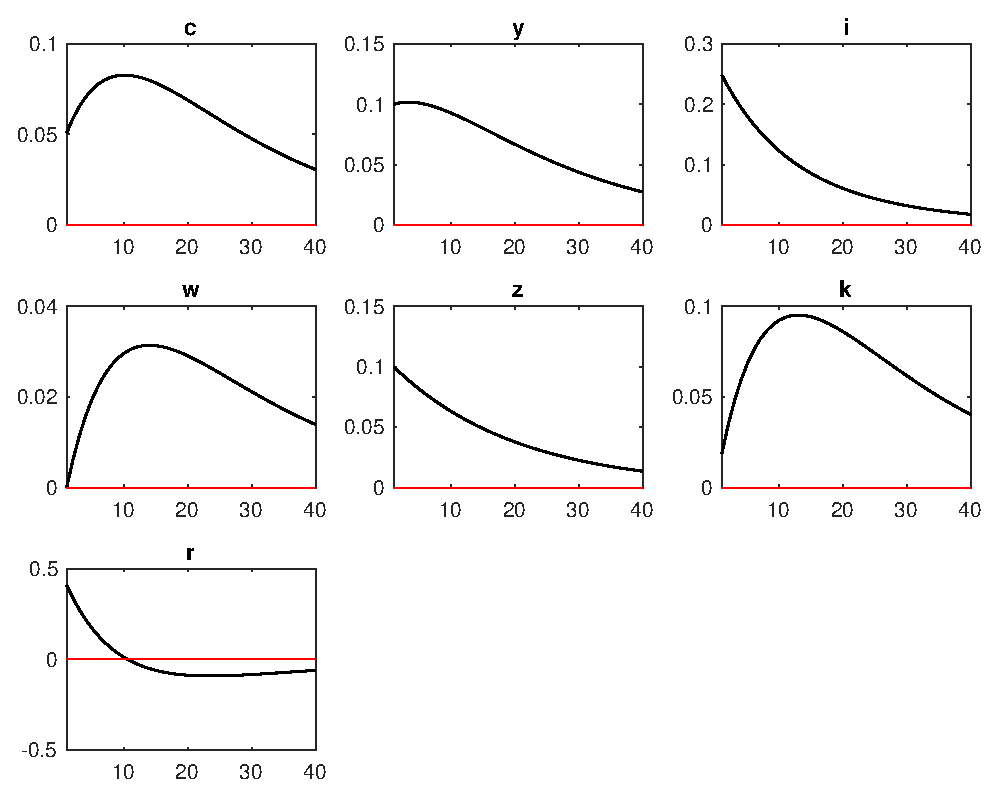
\includegraphics[width=1\textwidth]{Minki/Minki_dynare_IRF_epsilon.eps}
	\caption{Impulse responses from Dynare}
\end{figure}

As one would expect, the impulse response looks the same as it does for the simulation.



\end{document}

